\PassOptionsToPackage{pdfpagelabels=false}{hyperref}
\documentclass{article}
\usepackage{natbib}
\usepackage{hyperref}
\usepackage{url}
\usepackage{amssymb}
\usepackage{amsmath}
\usepackage{graphicx}
\usepackage{siunitx}
\usepackage{hhline}
\usepackage[titletoc,title]{appendix}
\usepackage[utf8]{inputenc}
\usepackage[margin=1in]{geometry}

\makeatletter
\newcommand*{\Appendixautorefname}{Appendix}
\newcommand{\specialcell}[2][c]{\begin{tabular}[#1]{@{}c@{}}#2\end{tabular}}
\newsavebox\CBox\def\textBF#1{\sbox\CBox{#1}\resizebox{\wd\CBox}{\ht\CBox}{\textbf{#1}}}\parindent=0pt
\sisetup{exponent-product = \cdot}
\setlength{\parskip}{0.8em}
\renewcommand\hyper@natlinkbreak[2]{#1}
\makeatother

\begin{document}

\title{Reproduction of A Decomposable Attention Model for Natural Language Inference}

\author{
  \textbf{Xingyi Xu} \\ University of Melbourne \\ \texttt{stevenxxiu@gmail.com} \and
  \textbf{Jey Han Lau} \\ IBM Research \\ \texttt{depthchargex@gmail.com} \and
  \textbf{Timothy Baldwin} \\ University of Melbourne \\ \texttt{tb@ldwin.net}
}
\maketitle

\begin{abstract}
Neural network models can be difficult to reproduce due to its many hyperparameters, initialization and training details. We attempted to reproduce the results of a paper ``A Decomposable Attention Model for Natural Language Inference'' for the stanford natural language inference dataset, using \texttt{tensorflow}. For the vanilla approach, we obtained an accuracy of 85.9\%, comparable to the paper's 86.3\%. However for the intra-sentence approach, we did not find an improvement, and instead found significant overfitting and obtained a lower accuracy of 85.7\%, in comparison to the paper's 86.8\%.
\end{abstract}

\section{Introduction}
The recent resurgence in AI is in large part due to the many successful neural network models. These models often have many hyperparameters, and can be initialized and trained in multiple ways. However, the focus on many papers has been just the model itself, with a minimal or neglected description of the details, possibly due to the fact that different initilization and training schemes can still achieve similar results. Hence it is useful to investigate whether we can reproduce neural network papers using its description alone, and if not, what can be done to improve reproducibility.

We investigate a paper in the space of natural language inference. This is the problem of given two sentences, determining whether sentence 2 entails (E), contradicts (C), or is neutral (N) to sentence 1. Examples are given in \autoref{table:examples}.

\begin{table}[htbp]\centering
\setlength\tabcolsep{2pt}
\begin{tabular}{|p{7.5cm}|p{7.5cm}|c|}
    \hline
    Sentence 1 & Sentence 2 & Label \\ \hhline{|===|}
    A man inspects the uniform of a figure in some East Asian country. & The man is sleeping & C \\ \hline
    An older and younger man smiling. & Two men are smiling and laughing at the cats playing on the floor. & N \\ \hline
    A black race car starts up in front of a crowd of people. & A man is driving down a lonely road. & C \\ \hline
    A soccer game with multiple males playing. & Some men are playing a sport. & E \\ \hline
    A smiling costumed woman is holding an umbrella. & A happy woman in a fairy costume holds an umbrella. & E \\ \hline
\end{tabular}
\caption{Examples from the Stanford Natural Langauge Inference (SNLI) dataset.}
\label{table:examples}
\end{table}

The paper ``A Decomposable Attention Model for Natural Language Inference'' \citep{parikh_decomposable_2016} is interesting in that despite being a model with a relatively low 580K parameters, it achieves a good claimed accuracy of 86.8\% on the SNLI dataset \citep{snli:emnlp2015}, which is not too far behind the current best model of 88.8\% accuracy, with 6.4M parameters. Another aspect is that the vanilla part of the model does not take any word ordering into account, however still manages to achieve a claimed accuracy of 86.3\%. For these reasons we decided to investigate this particular paper.

In the following sections, we give a description the vanilla and intra-sentence models, any ambiguities in the paper which slowed down our implementation, and a report of how we managed to implement the model.

\section{Models}
We found the model to be very well described, and the only part that may be unclear is the training objective's dropout being stated in the experimental section. We now describe the model for the purpose of being self-contained, and use the paper's notation.

Let the two input sentences be $\textbf{a}=(a_1,...,a_{l_a})$ and $\textbf{b}=(b_1,...,b_{l_b})$ with lengths $l_a$ and $l_b$, respectively. $a_i, b_j\in\mathbb{R}^d$ are word embeddings of dimension $d$ for word $i$ in sentence 1 and word $j$ in sentence 2. In the paper's experiments they are fixed GloVe vectors with some special treatment regarding OOV words and the \texttt{null} word. Now let $\bar{a}_i = a_i, \bar{b}_i = b_i$. The reason we use $\bar{a}_i, \bar{b}_i$ instead is for convenience in describing the intra-sentence approach, where they are different to $a_i, b_i$.

For the first step, we soft-align each word with the other sentence. Let $F$ be a feed-forward network with ReLU activations, and define the unnormalized attention weights $e_{i,j} := F(\bar{a}_i)^T F(\bar{b}_j)$. We normalize and perform a weighted sum:

\begin{align*}
    \beta_i := \sum_{j=1}^{l_b} \frac{\exp(e_{i,j})}{\sum_{k=1}^{l_b}\exp(e_{i,k})} \bar{b}_j &&
    \alpha_j := \sum_{i=1}^{l_a} \frac{\exp(e_{i,j})}{\sum_{k=1}^{l_a}\exp(e_{k,j})} \bar{a}_i
\end{align*}

For the second step, we compare soft alignment with their corresponding sentence. Let $G$ be a feed-forward network with ReLU activations, and define $\mathbf{v}_{1,i} := G([\bar{a}_i, \beta_i]), \mathbf{v}_{2,j} := G([\bar{b}_j, \beta_j])$ for $i=1,...,l_a, j=1,...,l_b$, where $[\cdot, \cdot]$ denotes concatenation.

For the third and last step, we aggregate the comparison vectors by summation $\mathbf{v}_1 = \sum_{i=1}^{l_a}\mathbf{v}_{1,i}, \mathbf{v}_2 = \sum_{j=1}^{l_b}\mathbf{v}_{2,i}$. Let $H$ be a feed-forward network with ReLU activations with a final softmax classification layer, we define the prediction $\hat{y} := H([\mathbf{v}_1, \mathbf{v}_2])$. Here $\hat{y}\in\mathbb{R}^C$ for $C$ classes.

Now given training instance $n$, for the prediction $\hat{y}_c^{(n)}$ and true binary labels $y^{(n)}\in\{0, 1\}^C$, the training objective is the categorical cross-entropy loss $L = \frac{1}{N} \sum_{n=1}^N \sum_{c=1}^C y_c^{(n)} \log \hat{y}_c^{(n)}$.

\subsection{Intra-sentence attention}
In the intra-sentence attention modification to the model, $\bar{a}_i, \bar{b}_i$ are defined differently. The modification aligns a sentence to itself. Let $F_\text{intra}$ be a feed-forward network with ReLU activations, and define the unnormalized alignment weights $f_{i,j} := F_\text{intra}(\bar{a}_i)^T F_\text{intra}(\bar{a}_j)$. Now for words at positions $i, j$, a distance sensitive bias $d_{i-j}\in\mathbb{R}$ is added to the weights to provide the model with sequence information. The bias is defined s.t. $d_{i-j} = d_\text{far}$ for $|i-j| > 10$, where $d_\text{far}$ is a trained parameter. The self-aligned phrases are:

\[a'_i := \sum_{j=1}^{l_a} \frac{\exp(f_{i,j} + d_{i-j})}{\sum_{k=1}^{l_a} \exp(f_{i,k} + d_{i-k})} a_j\]

And in place of the word embeddings, we use: $\bar{a}_i := [a_i, a_i'], \bar{b}_i := [b_i, b_i']$.

\subsection{Ambiguities common to most neural network papers}
The total loss is described, but not the batch loss. We assume that the batch loss is the loss restricted to instances within the batch.

\section{Experimental results}
In our reproduction of the vanilla approach, we obtained an accuracy of 85.9\%, comparable to the paper's 86.3\%. However for the intra-sentence approach, we did not find an improvement, and instead found significant overfitting and obtained a lower accuracy of 85.7\%, in comparison to the paper's 86.8\%.

\subsection{Ambiguities in the paper}
We now detail some unclear or unexplained parts of the paper.

What $F, F_\text{intra}, G, H$ are exactly is not specified. The paper described $F$ as a ``feed-forward network with ReLU activations'', and that the network size was ``$2$-layers, each with $200$ neurons''. It can be guessed that each of $F, F_\text{intra}, G, H$ are $2$-layer neural networks, each with $200$ neurons and ReLU activations, excluding $H$'s final linear layer.

The total number of parameters then approximately matches that given in the paper. For the vanilla approach, this is $300 \cdot 200 + (201 \cdot 200 + 201 \cdot 200) + (401 \cdot 200 + 201 \cdot 200) + (401 \cdot 200 + 201 \cdot 200 + 201 \cdot 3) = 381803 \approx 382\text{K}$, and for the intra-sentence approach, this is $300 \cdot 200 + 21 + (201 \cdot 200 + 201 \cdot 200) + (401 \cdot 200 + 201 \cdot 200) + (801 \cdot 200 + 201 \cdot 200) + (401 \cdot 200 + 201 \cdot 200 + 201 \cdot 3) = 582224 \approx 582\text{K}$.

The description of out-of-vocabulary (OOV) words is slightly unclear. We suppose it is any word that is not in the pretrained GloVe dataset \citep{pennington2014glove}. There were then a total of $4042 + 80 + 86 = 4208$ OOV words in the SNLI dataset, for train, val and test respectively. Most had spelling mistakes or were words joined with a hyphen.

We assume that the OOV vectors are also normalized to a $l_2$ norm of $1$ after their random initialization, as otherwise they would be on a different scale to the GloVe vectors, and we found this to produce worse results.

It is also unclear why there are $100$ random OOV vectors in the first place instead of just $1$ or OOV vectors simply being ommitted entirely. The prescence of many OOV vectors however will promote randomness, so we expect the results to be noisier. The exact hashing is not specified, and we used $\text{hash}(w) \mod 100$ as the word index, where hash is python's \texttt{hash} function (may differ depending on the python version).

It is unclear what the \texttt{null} word's embedding was initialized and whether it was trained. We supposed it is random and not trained like the other embeddings. There was no \texttt{null} word in the GloVe dataset.

The paper explicitly stated that they used ``the tokenized sentences from the non-binary parse provided in the dataset'', however we found no difference between the tokens of the binary parse and non-binary parse for each sentence, as was expected.

It is not explained why the authors decided to project the embeddings down from GloVe's pretrained $300$ dimensions to $200$ dimensions. Projection may serve some regularization effect. Denote the projection matrix $W_\text{proj}$ and the first layer of $F, G$'s weight be $W_F, W_G$, with $W_{G,1}, W_{G,2}$ the top and bottom halves of $W_G$. Then an equivalent network is $W_{F'} = W_\text{proj} W_F, W_{G',1} = W_\text{proj} W_{G,1}, W_{G',2} = W_\text{proj} W_{G,2}$. With arbitrary inputs to these 2 networks, this can be written as $[W_{F'}, W_{G',1}, W_{G',2}] = W_\text{proj} [W_F, W_{G',1}, W_{G',2}]$. We can see that LHS has rank $\le 300$ while RHS has rank $\le 200$. Empirically from \autoref{fig:test_no_proj_vs_proj}, this slightly reduces overfitting, despite having the same number of parameters.

The initialization of projection embeddings itself is unclear. We tried to initilize the same as other parameters, through $\mathcal{N}(0, 0.01)$, and also tried initializing them with the PCA transform matrix (in this case the embeddings are also centered first).

\subsection{Implementation details}
Due to our use of GPUs, it was easier for us to use one large batch size instead of the paper's ``10 asynchronous gradient-update threads''. We tried a similar setting with a batch size of $40$ with Adagrad, but we found that used Adam \citep{kingma_adam:_2014}, with a learning rate of $0.0005$ with a batch size of $256$, converged and ran faster, and attained a better result (\autoref{table:results}).

Usually when embedding vectors are trained, we only need to include words in the training set, but since embeddings are pretrained static GloVe vectors, we should include all words in the GloVe dataset. For efficiency this is the intersection between the set of GloVe words and all words in the SNLI dataset (this includes the training, validation and test sets). This detail can be missed in the implementation.

It may also be worth mentioning the way we implemented masking. We used a binary masking array for each batch. The masking array was used in the attend step (both intra and inter) to set the unnormalized weights being masked out to $-\infty$, so that corresponding outputs of the softmax are $0$. The masking array was used again in the aggregate step, in which comparison vectors being masked out were set to $0$ before being summed over.

\subsection{Results}
The results are presented in \autoref{table:results}. Using mean norm or different projection initializations do not appear to make a significant difference. Using the paper's AdaGrad and it's settings also do not perform as well.

From \autoref{fig:test_vanilla_vs_intra}, we can see that intra-sentence initially performs slightly better, but then becomes worse. This is likely due to overfitting, due to the initial rise in test performance and then the gradual decay.

\begin{table}[htbp]\centering
\begin{tabular}{|l|l|l|l|r|}
    \hline
    Method         & Embedding transform & Projection init & Update  & Accuracy \\ \hline
    vanilla        & norm                & Gaussian        & Adam    & 0.855558 \\
    vanilla        & mean norm           & Gaussian        & Adam    & \textBF{0.858917} \\
    vanilla        & mean norm           & PCA             & Adam    & 0.855252 \\
    intra-sentence & norm                & Gaussian        & Adam    & 0.856983 \\
    intra-sentence & mean norm           & Gaussian        & Adam    & 0.855863 \\
    intra-sentence & mean norm           & PCA             & Adam    & 0.856169 \\
    intra-sentence & norm                & Gaussian        & AdaGrad & 0.843139 \\
    \hline
\end{tabular}
\caption{Classification results for the SNLI dataset. For Adam we used a learning rate of $0.0005$, a batch size of $256$, and $400$ epochs. For AdaGrad we used a learning rate of $0.025$, a batch size of $40$, and $400$ epochs. We took the result of the best epoch on validation.}
\label{table:results}
\end{table}


\begin{figure}
\centering
\begin{minipage}[t]{.49\textwidth}
    \centering
    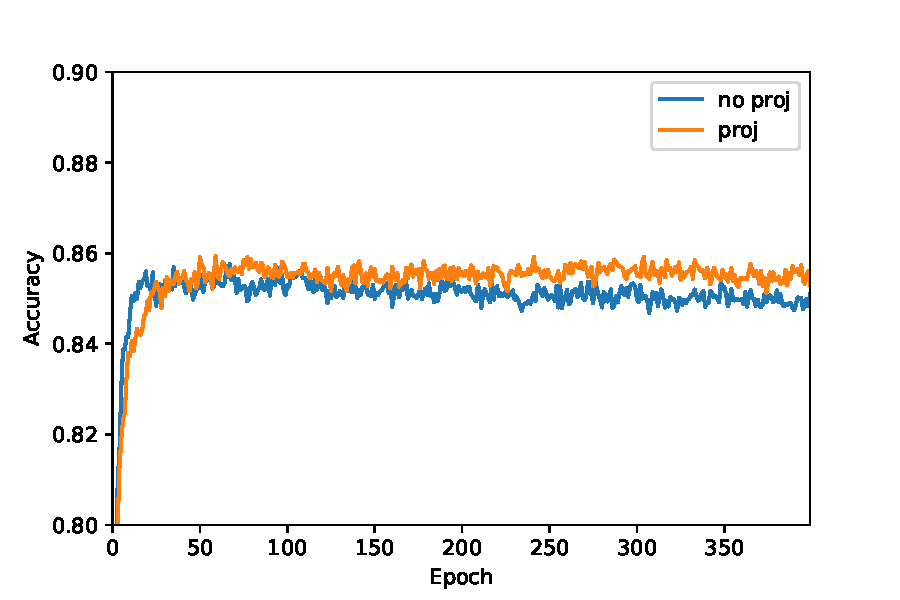
\includegraphics[scale=0.5]{fig/test_no_proj_vs_proj.pdf}
    \caption{Test accuracies for the vanilla model comparing no projection vs projection, both with normed embedding transforms.}
    \label{fig:test_no_proj_vs_proj}
\end{minipage}%
\hfill
\begin{minipage}[t]{.49\textwidth}
    \centering
    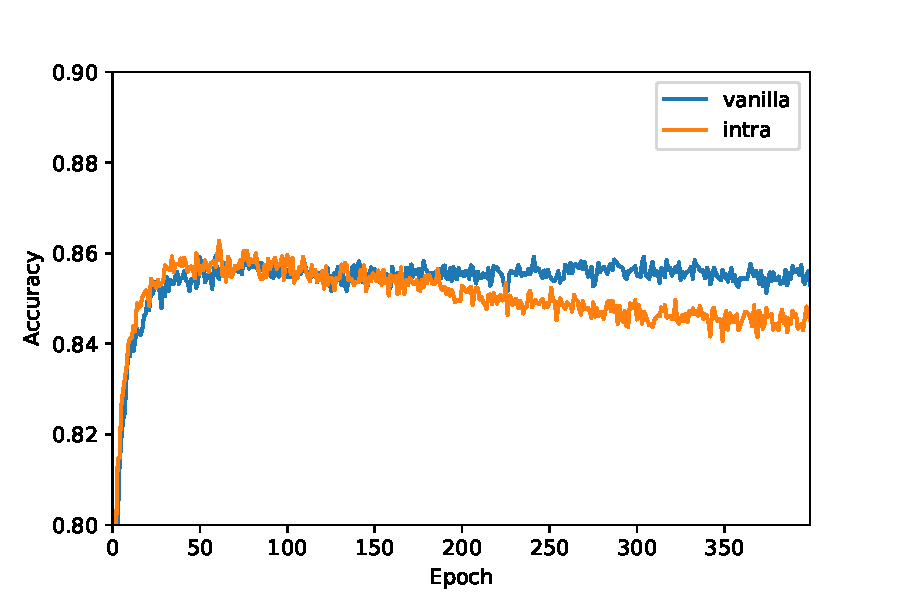
\includegraphics[scale=0.5]{fig/test_vanilla_vs_intra.pdf}
    \caption{Test accuracies for vanilla and intra-sentence models, both with normed embedding transforms.}
    \label{fig:test_vanilla_vs_intra}
\end{minipage}
\end{figure}

\section{Conclusion}
We have described the process in which we attempted to reproduce the paper ``Reproduction of A Decomposable Attention Model for Natural Language Inference''. The paper was in general well described and not difficult to reproduce. Issues include the slightly vague description of the network parameters, normalization and initialization of OOV and \texttt{null} vectors, and the initilization of the embedding projection matrix. The motivations behind the processing of OOV words can also be better described. We hope that our findings can guide future paper authors in the area of deep learning to describe their models in a clearer fashion so that they are more easily reproducible.

\bibliography{main}{}
\bibliographystyle{apalike}

\end{document}
